\documentclass[conference]{IEEEtran}

\usepackage{amsmath,amssymb}
\usepackage{booktabs}
\usepackage{graphicx}
\usepackage{float}
\usepackage{tikz}
\usetikzlibrary{arrows.meta,positioning}
\usepackage{xurl}
\usepackage[hidelinks]{hyperref}

\title{Q-OpCert: Bounded-Error Shadow and ABFT Checks for Instruction-Skip Resilience in CMSIS-NN}

\author{\IEEEauthorblockN{Anonymous Author(s)}}

\begin{document}
\maketitle

\begin{abstract}
Optimized integer neural-network kernels compress multiply--accumulate (MAC), requantization, checking, and output commit into short instruction sequences. An instruction skip can therefore corrupt an activation without causing an exception. This paper presents Q-OpCert, a software integrity mechanism for INT8 CMSIS-NN convolution. Q-OpCert combines a bounded-error shadow requantizer, a channel-checksum relation for the MAC path, exact output-address checks, and a dual-rail infective commit. Under stated arithmetic assumptions, an output accepted by the shadow checker differs from the fault-free exact output by at most two least-significant bits. On an STM32F407, shadow, shadow+ABFT, and dual-rail state add 1.778\%, 5.348\%, and 5.445\% cycles. On STM32U575, shadow and shadow+ABFT add 10.328\% and 33.580\%; the final design, including writeback and pointer checks, adds 44.040\%. A board-level campaign replaced every enumerated instruction in the protected M33 code surface with an equal-width NOP sequence. Across three convolution profiles, 1,971 mutant images produced 229,525 recorded trials. The campaign exposed five blind-spot classes in output writeback, pointer integrity, and checker metadata. After repair and complete re-enumeration, no trial produced an accepted error above the two-LSB bound. The result establishes exhaustive static-site coverage for the enumerated binaries and profiles, not physical injection coverage or general fault tolerance.
\end{abstract}

\begin{IEEEkeywords}
algorithm-based fault tolerance, CMSIS-NN, fault injection, instruction skip, quantized neural networks, software fault tolerance
\end{IEEEkeywords}

\section{Introduction}
Integer-only inference enables neural networks on microcontrollers with tight latency and memory budgets. CMSIS-NN supplies optimized kernels for this setting and implements the quantization conventions used by TensorFlow Lite for Microcontrollers~\cite{lai2018cmsisnn,jacob2018quantization,armcmsisnn}. Optimization, however, concentrates an output activation into a small number of MAC, requantization, clamp, and store instructions. Skipping one such instruction can corrupt an activation without raising a conventional exception.

Physical fault injection can induce software-visible instruction skips or more complex effects~\cite{barenghi2012fault,moro2014experimental,dutertre2021multiskip}. Neural-network implementations are also meaningful targets: faults in code, parameters, or intermediate activations can alter inference behavior~\cite{breier2018deeplaser,yao2020deephammer}. Gaine et al. demonstrated laser and electromagnetic instruction-skip attacks against Cortex-M4 neural-network inference, including a CMSIS-NN convolution path~\cite{gaine2023embedded}. Their work establishes the concrete attack surface; ours asks whether a kernel-level software mechanism can enforce a bounded-output contract under a defined static mutation model. Duplicating an entire layer is a simple defense, but it approximately duplicates its dominant work. Checking only the output epilogue is cheaper, yet shares the MAC accumulator with the main path and therefore cannot independently detect an erroneous dot product.

Q-OpCert addresses these two regions differently. A heterogeneous \texttt{SMMULR}-based shadow checks requantization and output formation with a bounded tolerance. A channel checksum independently recomputes a linear summary of the pre-requantization accumulators. Both syndromes feed an infective commit. We further treat the syndrome update itself as an attack surface: a complementary pair of sticky rails is independently updated so that omission of either tested update cannot erase the other.

This paper makes four contributions:
\begin{itemize}
  \item We derive a one-LSB bound between exact two-stage requantization and a shorter heterogeneous shadow, which implies a two-LSB bound for an accepted output.
  \item We integrate the shadow into official CMSIS-NN \texttt{arm\_convolve\_s8}, add a pre-requantization channel-checksum invariant, and protect output stores with readback and exact-address checks.
  \item We identify five blind-spot classes through a stop-on-silent repair loop. The classes separate computation faults from writeback-action, in-range pointer, cross-call pointer, and checker-metadata faults.
  \item We report costs on STM32F407 and STM32U575, then evaluate all 1,971 enumerated instruction sites in three M33 binaries. The repaired implementation has zero silent violations in 229,525 recorded trials.
\end{itemize}

The contribution is a software mechanism and deterministic mutation study. ``All sites'' below means the enumerated instruction set in the three linked M33 binaries, not all possible faults. We do not claim a physical injection success probability, model-level accuracy preservation, or generality beyond the evaluated boards and configurations.

\section{Background and Related Work}
\subsection{Quantized Inference on Cortex-M}
Integer-only inference maps a 32-bit accumulator back to INT8 using a quantized multiplier, a shift, an output offset, and activation clamping~\cite{jacob2018quantization}. CMSIS-NN specializes these operations and uses Cortex-M DSP instructions in optimized convolution paths~\cite{lai2018cmsisnn,armcmsisnn,armcortexm4}. Q-OpCert exploits architectural diversity within the same core: the main path retains the library's exact requantization, while the shadow uses rounded high-word multiplication.

\subsection{Fault Models and Software Countermeasures}
The instruction-skip abstraction is widely used to evaluate software countermeasures because it represents a recurring software-visible effect of several physical mechanisms~\cite{barenghi2012fault,moro2014experimental}. Formally verified replacement sequences can harden individual Thumb-2 instructions against one skip~\cite{moro2014formal}. Software defenses also include control-flow checking and redundant computation; SWIFT is a representative compiler-based redundancy scheme~\cite{reis2005swift}. Experiments have shown that one physical perturbation can affect multiple instructions, so a design validated only under an isolated single skip may retain exploitable decision points~\cite{dutertre2021multiskip}. This motivates our separate compound-skip stress tests, while not equating static double mutation with a physical double-fault probability.

\subsection{Fault Tolerance for Neural-Network Computation}
Prior work has demonstrated physical faults against embedded neural-network activation code, Cortex-M instruction flow, and network parameters~\cite{breier2018deeplaser,gaine2023embedded,yao2020deephammer}. Algorithm-based fault tolerance has been adapted to convolution through checksum identities, offering detection without duplicating every multiply~\cite{zhao2021ftcnn}. Gaine et al. characterize the impact of physical single skips but do not propose a bounded-output kernel defense. FT-CNN targets soft-error resilience in larger inference systems. Q-OpCert instead studies instruction omissions in an INT8 microcontroller kernel, combines an approximate output checker with an accumulator checksum, and hardens the checker state after observing a compound bypass.

\section{Q-OpCert Design}
Figure~\ref{fig:architecture} shows the protection boundaries. The shadow and ABFT paths observe different arithmetic stages. Store readback and pointer checks bind the arithmetic result to its memory destination. All evidence reaches two sticky rails before the infective commit decides whether the caller may accept the output.

\begin{figure}[H]
\centering
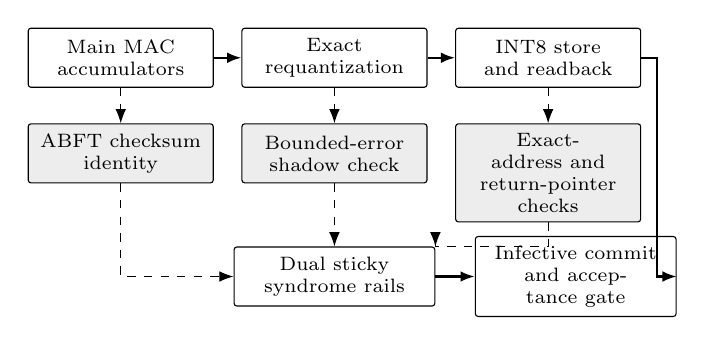
\begin{tikzpicture}[
  font=\scriptsize,
  node distance=4.5mm and 3.5mm,
  block/.style={draw, rounded corners=1pt, align=center, minimum height=7.5mm,
                text width=2.15cm, inner xsep=1mm},
  check/.style={block, fill=black!7},
  final/.style={block, text width=2.35cm},
  flow/.style={-{Latex[length=1.8mm]}, thick},
  evidence/.style={-{Latex[length=1.8mm]}, dashed}
]
\node[block] (mac) {Main MAC\\accumulators};
\node[block, right=of mac] (req) {Exact\\requantization};
\node[block, right=of req] (store) {INT8 store\\and readback};
\node[check, below=of mac] (abft) {ABFT checksum\\identity};
\node[check, below=of req] (shadow) {Bounded-error\\shadow check};
\node[check, below=of store] (addr) {Exact-address and\\return-pointer checks};
\node[final, below=8mm of shadow] (rails) {Dual sticky syndrome rails};
\node[final, right=5mm of rails] (commit) {Infective commit\\and acceptance gate};
\draw[flow] (mac) -- (req);
\draw[flow] (req) -- (store);
\draw[evidence] (mac) -- (abft);
\draw[evidence] (req) -- (shadow);
\draw[evidence] (store) -- (addr);
\draw[evidence] (abft.south) |- (rails.west);
\draw[evidence] (shadow) -- (rails);
\draw[evidence] (addr.south) -- ++(0,-3mm) -| (rails.north east);
\draw[flow] (rails) -- (commit);
\draw[flow] (store.east) -- ++(2mm,0) |- (commit.east);
\end{tikzpicture}
\caption{Q-OpCert protection boundaries. Solid arrows carry outputs or acceptance state; dashed arrows carry independent checker evidence.}
\label{fig:architecture}
\end{figure}

\subsection{Evaluation Fault Model and Safety Contract}
The primary campaign replaces one selected 16-bit Thumb instruction with one 16-bit NOP, or one selected 32-bit Thumb-2 instruction with two 16-bit NOPs. Targets include arithmetic, calls, comparisons, branches, syndrome updates, output stores, and commit operations. Availability failures are recorded separately from numerical integrity failures.

Let $Q_e$ be the fault-free exact output, $Q_o$ the observed main-path output, and $Q_s$ the independently formed shadow output. The output checker accepts a lane when
\begin{equation}
 |Q_o-Q_s|\leq 1.
 \label{eq:accept}
\end{equation}
Conditional on a fault-free shadow computation and comparison, the intended numerical contract is
\begin{equation}
 \text{reject}\quad\lor\quad |Q_o-Q_e|\leq2.
 \label{eq:contract}
\end{equation}
The ABFT relation adds exact detection for a non-cancelling error in its protected linear summary, subject to 32-bit arithmetic remaining in range. A conservative bound from the profile dimensions and declared input, weight, and bias ranges keeps both sides below $2^{17}$ in magnitude. Compound mutations are a second, stronger robustness probe. They test whether one main-path skip plus one checker-state skip can violate acceptance; they are not included in the single-skip detection rate.

\subsection{Bounded-Error Shadow Requantization}
For signed product $p=xm$, write the main path's doubling-high result as
\begin{equation}
 H=\left\lfloor\frac{p+2^{30}}{2^{31}}\right\rfloor.
\end{equation}
The rounded high-word instruction computes
\begin{equation}
 M=\left\lfloor\frac{p+2^{31}}{2^{32}}\right\rfloor,
\end{equation}
and the shadow uses $S=2M$. Writing $p=q2^{32}+r$, $0\leq r<2^{32}$, and partitioning $r$ at $2^{30}$, $2^{31}$, and $3\cdot2^{30}$ gives $H-S\in\{-1,0,1\}$. The evaluated per-channel shift is either $-3$ or $-4$; no left shift or undefined-width shift occurs. In this domain, the subsequent rounded division in the exact path and arithmetic shift in the shadow preserve
\begin{equation}
 |Q_e-Q_s|\leq1.
 \label{eq:shadow}
\end{equation}
The common output offset preserves the difference and saturation is non-expansive. Equations~\eqref{eq:accept} and~\eqref{eq:shadow}, with the triangle inequality, imply~\eqref{eq:contract}. An exhaustive executable check over 6,292,480 legal intermediate/shift combinations for the implemented convention observed a maximum exact--shadow difference of one LSB. The artifact records the checked domain and program. This result does not extend to other requantization conventions or shift domains.

\subsection{Channel-Checksum ABFT}
For one im2col input column $x$, output-channel weights $W$, and biases $b$, the pre-requantization accumulator is
\begin{equation}
 a_o=b_o+\sum_i W_{o,i}x_i.
\end{equation}
Summing over the four output channels yields
\begin{equation}
 \sum_o a_o=\sum_o b_o+\sum_i\left(\sum_o W_{o,i}\right)x_i.
 \label{eq:abft}
\end{equation}
The left side is accumulated from the main kernel's four channel accumulators. The right side is recomputed using a precomputed weight checksum and summed bias. Equality is checked independently for each of the two im2col columns processed by the DSP kernel. A single erroneous MAC that changes one protected accumulator therefore changes the left side and is detected; multiple errors whose signed effects cancel in the sum can escape this relation.

\subsection{Writeback and Pointer Integrity}
The arithmetic checks do not by themselves prove that the checked byte reached the intended output address. Q-OpCert therefore reads each stored output through a volatile-qualified pointer before comparison. This prevents the compiler from replacing the observed load with the requantized register value. The checker also reconstructs the exact address expected for each lane from a monotonic check index, the output base, and the output-channel count. It rejects both out-of-range pointers and in-range substitutions between adjacent output cursors.

The matrix-multiplication kernel returns an advanced output pointer to \texttt{arm\_convolve\_s8}. A separate caller-level check compares this return value with the expected offset before a later kernel invocation can use it. These checks cover three distinct events: execution of the store, selection of the destination element, and preservation of the output cursor across calls. The address reconstruction follows the kernel's global spatial order. It does not insert a per-row leftover element when the output width is odd.

\subsection{Sticky Syndrome and Infective Commit}
The output and ABFT checks set bits in a sticky syndrome. A nonzero syndrome is passed to two four-byte infective commits, which corrupt both output blocks and complement caller-held epochs. Acceptance requires both epochs to remain unchanged. The epochs, rather than the cleared output alone, are the final gate.

The initial ABFT implementation used one zero-initialized syndrome word. A main MAC skip combined with omission of either its comparison or syndrome store bypassed that state. The hardened design maintains primary rail $E$, initialized to zero and updated only by OR, and inverse rail $E_n$, initialized to all ones and updated only by bit clearing. Separate non-inlined functions update each rail. The final value is
\begin{equation}
 E_f=E\,\lor\,\neg E_n\,\lor\,(E\oplus\neg E_n),
\end{equation}
so either asserted rail or a rail mismatch causes rejection. This construction addresses omission of one tested rail update; coordinated corruption of both rails or the final reduction remains outside the demonstrated coverage.

\section{Experimental Method}
\subsection{Platform, Workload, and Measurement}
The cost study used an STM32F407VET6 with an Arm Cortex-M4 DSP core and Clang/LLD for Thumb-2 at \texttt{-Oz}. The full-site campaign used a NUCLEO-U575ZI-Q with an STM32U575 Cortex-M33, GNU Arm, \texttt{-O2 -g3}, hard-float FPv5, and \texttt{ARM\_MATH\_DSP}. The hardened build enabled all three checker channels. STM32CubeProgrammer 2.23.0 flashed each mutant over SWD at 8~MHz. Both bare-metal harnesses used USART CSV output and DWT \texttt{CYCCNT} timing. The timed region includes checker reset and configuration, convolution, syndrome retrieval, and infective commit as applicable. Input generation, the golden oracle, and UART output are outside it.

The integrated workload uses official CMSIS-NN v7.0.0, commit \texttt{22080c68}, and signed INT8 convolution. The cost study uses input $4\times5\times8$, filter $4\times4\times8$, and output $1\times2\times4$. The full-site study adds two shapes so that repeated kernel calls and an odd output width are exercised (Table~\ref{tab:profiles}). A separate scalar oracle validates every output but is not part of the run-time defense. Each mutant attempts the same 128 deterministic trials. Trial $t$ sets input element $i$ to $((17i+13t+5)\bmod31)-15$; fixed formulas generate weights, biases, multipliers, and shifts. This set is neither random sampling nor an exhaustive input space. A hang or early termination yields fewer records and is retained as an availability outcome.

\begin{table}[t]
\caption{Cortex-M33 Full-Site Convolution Profiles}
\label{tab:profiles}
\centering
\begin{tabular}{lccc}
\toprule
Profile & Input $(H,W,C)$ & Kernel $(H,W)$ & Output $(H,W,C)$\\
\midrule
p0 & $(4,5,8)$ & $(4,4)$ & $(1,2,4)$\\
p1 & $(5,6,8)$ & $(3,3)$ & $(3,4,8)$\\
p4 & $(5,5,8)$ & $(3,3)$ & $(3,3,8)$\\
\bottomrule
\end{tabular}
\end{table}

We compare baseline, fused shadow, an exact epilogue checker, shadow+ABFT, and hardened shadow+ABFT. ``Exact epilogue'' means exact requantization recomputed from the shared accumulator; it is not full convolution duplication. Percent overhead always uses the corresponding rebuilt baseline. The fused and ABFT harness baselines differ by four cycles because their instrumentation and layout differ.

\subsection{Mutation Campaigns and Outcome Classes}
The linked ELF was patched at selected instruction addresses and disassembled again to confirm equal-width NOP replacement. The legacy microkernel campaign contains 62 priority-one mutants across ten phases. Mode 12 is the end-to-end numerical harness; modes 10 and 11 are aggregate component self-tests and are not used to claim a detection rate.

The final M33 campaign parses GNU \texttt{objdump} output for seven named linked functions: the main matrix kernel, shadow check, ABFT check, both rail latches, syndrome reduction, and commit. Every parsed 16- or 32-bit instruction in those function bodies becomes one manifest row; its address and original bytes are checked against the linked binary. No dynamic-coverage filter is applied. Each 16-bit instruction is replaced by \texttt{00bf}; each 32-bit instruction is replaced by two 16-bit NOPs so that addresses do not shift. The mutated image is disassembled and flashed before capture. The denominator is 657 sites per profile, or 1,971 profile-site pairs. It contains 1,506 main-kernel/control sites, 243 shadow sites, 132 ABFT sites, 24 commit sites, and 66 rail or reduction sites.

For each recorded trial, \emph{erroneous} means the maximum absolute error against the scalar oracle is nonzero. \emph{Rejected} means the final acceptance gate is false. A \emph{bounded accept} is accepted with an error of one or two LSB. A \emph{silent violation} is accepted with an error above two LSB. The campaign stops immediately with a distinct nonzero exit status if any silent violation occurs. After a repair, we rebuild, re-enumerate, regenerate every mutant, and restart the three-profile campaign. COMPLETE, PARTIAL, and HANG status are reported separately.

\section{Results}
\subsection{Bounded-Error Microkernel Campaign}
All 62 mutant images produced saved board records. Fifty-nine completed 128 trials; two skipped returns produced only the header, and one skipped loop comparison stopped after three trials. These are availability outcomes, not missing experiments. No complete or partial record reported a HardFault.

The end-to-end subset contains 25 mutants and 3,200 trials. Of 2,011 trials with nonzero error, 1,925 were rejected. The remaining 86 accepted errors were exactly one LSB: 43 from one MAC-body mutant and 43 from one clamp-related mutant. No accepted trial exceeded the two-LSB contract (Table~\ref{tab:micro}). The 95.7\% rejection fraction describes these fixed activated outcomes; it is not a physical attack-detection probability.

\begin{table}[t]
\caption{End-to-End Microkernel Mutation Results}
\label{tab:micro}
\centering
\begin{tabular}{lrrrr}
\toprule
Phase & Trials & Error & Rejected & Accepted $>2$\\
\midrule
Clamp & 512 & 340 & 297 & 0\\
Loop control & 640 & 214 & 214 & 0\\
MAC body & 1,024 & 730 & 687 & 0\\
Output commit & 512 & 512 & 512 & 0\\
Requant. call & 512 & 215 & 215 & 0\\
\midrule
Total & 3,200 & 2,011 & 1,925 & \textbf{0}\\
\bottomrule
\end{tabular}
\end{table}

\subsection{Integrated CMSIS-NN Cost}
All clean builds completed 128/128 trials with zero numerical error, zero syndrome, no crash marker, and identical trial-by-trial output checksums. Table~\ref{tab:cost} reports the measured design points. Fused shadow checking adds 767 cycles (1.778\%), compared with 855 cycles (1.982\%) for the exact epilogue checker. Shadow+ABFT adds 2,307 cycles (5.348\%). Dual-rail hardening adds only 42 cycles over that design, for 5.445\% total overhead.

\begin{table}[t]
\caption{STM32F407 Integrated-Layer Cost}
\label{tab:cost}
\centering
\begin{tabular}{lrrr}
\toprule
Build & Cycles & Text (B) & BSS (B)\\
\midrule
Fused baseline & 43,134 & 5,304 & 1,260\\
Fused shadow & 43,901 & 5,798 & 1,268\\
Exact epilogue & 43,989 & 5,765 & 1,268\\
ABFT baseline & 43,138 & 5,410 & 1,260\\
Shadow+ABFT & 45,445 & 6,157 & 1,544\\
Hardened ABFT & 45,487 & 6,230 & 1,548\\
\bottomrule
\end{tabular}
\end{table}

Relative to its baseline, the hardened design adds 820 B of text (15.16\%) and 288 B of BSS. Of the BSS increase, 256 B holds prototype checksum weights that are immutable after model loading and can be stored as Flash model metadata. We report the measured BSS rather than subtracting this optimization prospectively.

\subsection{Cortex-M33 Replication}
The five initial STM32U575 clean images completed 128/128 trials with exact outputs, identical checksums, zero syndromes, and no crash. Table~\ref{tab:m33} reports medians against the matched M33 baseline; absolute cycle counts are not compared across boards because the MCU and compiler configurations differ. The shadow remained cheaper than exact epilogue recomputation, while ABFT dominated the incremental cost. Dual-rail state added 39 cycles over shadow+ABFT. After the repair loop added writeback and pointer checks, the no-op mutant of the final p0 binary reproduced the clean binary hash and measured 7,601 median cycles over 128 trials. The final overhead is therefore 44.040\%, rather than the pre-address-check value of 34.319\%.

\begin{table}[t]
\caption{STM32U575 Cortex-M33 Integrated-Layer Cost}
\label{tab:m33}
\centering
\begin{tabular}{lrrr}
\toprule
Build & Cycles & Overhead & Text/BSS (B)\\
\midrule
Baseline & 5,277 & 0\% & 22,400/3,376\\
Shadow & 5,822 & 10.328\% & 22,968/3,664\\
Exact epilogue & 5,934 & 12.450\% & 22,928/3,664\\
Shadow+ABFT & 7,049 & 33.580\% & 23,136/3,664\\
Dual rail, pre-address checks & 7,088 & 34.319\% & 23,208/3,664\\
Final Q-OpCert & 7,601 & 44.040\% & 23,600/3,696\\
\bottomrule
\end{tabular}
\end{table}

These measurements establish the cost of the clean mechanisms before the full-site campaign. The campaign results below use the hardened build only and should not be interpreted as a detection-rate comparison among the five cost-study builds.

\subsection{Complete M33 Static-Site Campaign}
Table~\ref{tab:date} reports the final campaign after all repairs. Every profile completed all 657 mutants. HANG denotes an image that produced no trial rows before the capture deadline; PARTIAL denotes early termination after at least one row. The 1,971 images produced 229,525 recorded trials rather than the nominal 252,288 because 171 images hung and nine terminated early. None of the recorded trials was a silent violation.

\begin{table}[t]
\caption{Final Cortex-M33 Full-Site Campaign}
\label{tab:date}
\centering
\begin{tabular}{lrrrrrr}
\toprule
 & Sites & Complete & Partial & Hang & Trials & Silent\\
\midrule
p0 & 657 & 598 & 3 & 56 & 76,655 & 0\\
p1 & 657 & 596 & 3 & 58 & 76,335 & 0\\
p4 & 657 & 597 & 3 & 57 & 76,535 & 0\\
\midrule
Total & 1,971 & 1,791 & 9 & 171 & 229,525 & \textbf{0}\\
\bottomrule
\end{tabular}
\end{table}

Across the recorded trials, 99,111 had nonzero numerical error, 85,239 were rejected, and 14,256 were bounded accepts. These counts overlap because a rejected trial can have a zero output error after infective clearing, and an erroneous trial can also be rejected. The categories are predicates, not a partition. All 14,256 bounded accepts came from the main-kernel/control group. ABFT, shadow, rail, reduction, and commit sites produced no accepted erroneous output.

\subsection{Blind Spots Found During the Repair Loop}
The stop-on-silent rule exposed five failure classes before the final run (Table~\ref{tab:blind}). First, an optimized store followed by an apparent readback reused the register value; skipping the store left memory stale while the shadow still passed. A volatile readback forced observation of the buffer. Second, a damaged output cursor could point into valid SRAM outside the output range. A range check rejected it. Third, corruption of the kernel's returned cursor affected the next call but escaped checks inside the current call. A caller-level expected-return check closed this gap.

The fourth class remained after range checking: two adjacent output cursors were both in range, so substituting one for the other required an exact expected-address check. The first implementation of this check introduced the fifth class. It assumed that an odd output width inserted one leftover column per row. CMSIS-NN advances the pair counter globally, so the formula falsely asserted the syndrome throughout p4. Skipping the epoch complement in commit then converted that false rejection into an accepted erroneous result. Removing the per-row leftover term restored continuous spatial addressing. A fresh three-profile run, not a selective replay, produced Table~\ref{tab:date}.

\begin{table}[t]
\caption{Blind-Spot Taxonomy and Repairs}
\label{tab:blind}
\centering
\footnotesize
\begin{tabular}{p{0.20\columnwidth}p{0.31\columnwidth}p{0.34\columnwidth}}
\toprule
Blind spot & Failure mechanism & Repair\\
\midrule
Store omission & Compiler reused register & Volatile memory readback\\
Range escape & Arithmetic remained correct & Output-range check\\
Return cursor & Error affected the next call & Caller-level offset check\\
Address alias & Both pointers were in range & Exact element address\\
Metadata model & Odd-width formula was wrong & Continuous spatial index\\
\bottomrule
\end{tabular}
\end{table}

\subsection{Integrated Fault Activation and Hardening}
The two representative main-path \texttt{SMLAD} skips activated on every input. The ABFT relation rejected all 256 activated trials, with no accepted error. Skipping the main channel-sum update also activated and rejected 128/128 trials. A skip in the independent checksum dot product produced 128/128 safe rejections, demonstrating fail-safe behavior but also a potential availability cost. The clean-path comparison and syndrome-store skips did not activate; they are counted as masked, not detected.

The compound controls expose why that distinction matters. Combining the activated main-MAC skip with either the comparison skip or syndrome-store skip suppressed the original ABFT evidence. Both images silently accepted all 256 erroneous trials, whose maximum absolute errors ranged from 1 to 47 LSB (mean 22.211). Thus, the original checker had a demonstrated single-state bypass under the compound model.

The hardened clean image retained exact output in 128/128 trials. In four regressions, the same main-MAC error was paired with omission of the primary comparison call, secondary comparison call, primary state store, or secondary state store. The intact rail asserted the final syndrome and all 512 trials were rejected, with zero silent acceptance and no crash. Table~\ref{tab:faults} separates the three evidential scopes.

\begin{table}[t]
\caption{Integrated-Kernel Fault Evidence}
\label{tab:faults}
\centering
\begin{tabular}{lrrr}
\toprule
Campaign & Activated & Rejected & Silent\\
\midrule
Main MAC, single skip & 256 & 256 & 0\\
Original state, compound & 256 & 0 & 256\\
Dual rail, compound regression & 512 & 512 & 0\\
\bottomrule
\end{tabular}
\end{table}

\section{Discussion}
The results support three linked claims. First, heterogeneous output checking can be fused into a real optimized convolution and remains cheaper than exact epilogue recomputation on both evaluated cores. Second, the channel checksum extends protection upstream to MAC faults, although its relative cost is platform dependent: shadow+ABFT costs 5.348\% on the F407 and 33.580\% on the U575. The output-action and pointer repairs raise the final U575 overhead to 44.040\%. Third, arithmetic redundancy alone does not protect output delivery. Three of the five blind spots affected the store or a pointer after the checked arithmetic was already correct. The final mechanism must bind a checked value to its memory effect and to the cursor that determines later effects.

The shadow and ABFT provide different contracts. The shadow intentionally tolerates a one-LSB arithmetic discrepancy and offers the deterministic accepted-error bound in~\eqref{eq:contract}. The ABFT relation is exact for its checksum but structurally incomplete: signed errors can cancel, and faults in both the main summary and checksum computation can agree incorrectly. Exact-address and return-pointer checks cover a different boundary. Their combination explains the zero-silent result for the enumerated campaign, but it is not a proof for unenumerated fault effects.

Availability is also distinct from integrity. Three legacy mutants failed to complete, and a checksum-path fault safely rejected correct main computation. A deployable system should pair Q-OpCert with a watchdog and persistent progress state; otherwise, fail-stop behavior remains visible only as missing service.

\subsection{Limitations and Validity Threats}
Static ELF mutation precisely reproduces selected instruction omissions but not the timing, spatial spread, instruction replacement, register corruption, or success distribution of laser, electromagnetic, clock, or voltage injection. The selected sites are not a random sample, so trial ratios must not be generalized to all instructions or physical attempts.

The cost evidence covers one small convolution on each board. The full-site evidence covers three shapes, one Cortex-M33 compiler configuration, and one optimized CMSIS-NN path. Exhaustiveness applies only to the instructions enumerated in those three linked binaries. Static replacement does not reproduce the timing or spatial distribution of a physical disturbance, and it cannot model register corruption, instruction replacement, or a multi-instruction effect unless those effects are separately constructed.

The study does not evaluate a complete network, model-level accuracy, other CMSIS-NN kernels, TrustZone-enabled execution, energy, or physical injection. The 128 deterministic inputs per image exercise repeatable data-dependent paths but do not estimate a workload distribution or exhaust dynamic states. HANG and PARTIAL outcomes establish loss of availability, not numerical safety after recovery or reuse of a partly written buffer. Absolute cycles are not comparable across boards and toolchains; the 44.040\% U575 result is for this small convolution and prototype implementation. The arithmetic proof assumes the implemented two-stage requantization and stated shift domain; the ABFT equality cannot detect cancelling error patterns. Finally, the repair loop used observed counterexamples to strengthen the mechanism. The final complete rerun avoids selective validation, but independent reproduction on another toolchain remains necessary.

\section{Conclusion}
Q-OpCert combines bounded-error shadow requantization, a channel-checksum MAC invariant, output-action and pointer checks, and a dual-rail infective commit for INT8 CMSIS-NN. On STM32F407, shadow, shadow+ABFT, and dual-rail state add 1.778\%, 5.348\%, and 5.445\% cycles. On STM32U575, the final mechanism adds 44.040\% against the matched baseline. The complete M33 campaign evaluated 1,971 profile-site pairs and recorded 229,525 trials. It found five blind-spot classes during development. After repair and full re-enumeration, no recorded trial silently violated the two-LSB contract. The main lesson is narrower than complete fault tolerance: protecting arithmetic is insufficient unless the checker also verifies the output store, exact destination, cross-call cursor, and its own metadata assumptions.

\section*{Data Availability}
The anonymous artifact provides source code, build and mutation scripts, the complete site denominator, final board records, and a portable result verifier at \url{https://anonymous.4open.science/r/Q-OpCert-BDC8}.

\section*{Acknowledgment}
OpenAI Codex assisted with language editing and consistency checks throughout the manuscript. It did not design or execute the experiments. The authors inspected the source data, verified every reported result, and retain responsibility for the manuscript. Project acknowledgments are omitted for double-blind review.

\bibliographystyle{IEEEtran}
\bibliography{references}
\end{document}
